\chapter{Systematic Errors Study}
\resetfootnote

\pagestyle{fancy}
\markboth{\bfseries \slshape Systematics}{}
\renewcommand{\sectionmark}[1]{\markright{\bfseries \slshape \thesection\ #1}{}}
\fancyhead[R]{\rightmark} 
\fancyhead[L]{\leftmark}
\fancyfoot[L]{}
\fancyfoot[R]{\sl Maurizio Ungaro}


\section{ Calculation of the c.m. angle $\theta^*$ }\label{sec:cmsyst}

The $\pi^0$ c.m. angle $\theta^*$ can be calculated in two ways:


\begin{itemize}
 \item[1)] {\bf Lorentz method:} using the four vectors of the final electron and proton, 
           one can calculate the c.m. four vectors with a lorentz transformation from the lab to the c.m.
 \item[2)] {\bf boost method:} assuming the reaction is a $\Delta \rightarrow \pi^0 P$, one can calculate
            the momentum of the proton in the C.M frame using just the electron four vector and kinematics.
\end{itemize}

Previous analysis of lower energy data showed that the systematic on the proton reconstruction favors method 2), as it is independent 
of the proton detection. However this method is also more affected by radiation of the electron. Monte Carlo studies
below show that the Lorentz method gives better results. 


\subsection{The Lorentz Method}
As described in Appendix \ref{sec:kinema},  $H_{\mu}$ is the outgoing hadrons mass four vector 
$H_{\mu}=q_{\mu}+P_{\mu}$ ($W=\sqrt{H_\mu H^\mu}$), where 
$q_{\mu}= e_{\mu}-e_{\mu}'$ (all quantities in the lab).
The $\pi^0$ lab four vector is $x_{\mu}=H_{\mu}-P_{\mu}'$.

In \F{fig:kinema} is illustrated the definition of the angles $\phi^*$ and $\theta^*$.
%To obtain $x^{cm}_\mu$, one must first rotate the lab frame of $\phi(H)$ + $180^0 $ (see \F{fig:kinema},
%then align the z-axis to the virtual photon direction, and finally perform a boost:
To obtain $x^{CM}_\mu$ we can rotate the lab frame in order to overlap the $z-axis$ with the $\vec{q}$ direction,
then perform a $\beta = (t, x, y, z) = (0, 0, 0, |\vec{H}|/H_0)$ lorentz boost
$x'_\mu = \Lambda(\beta)_\mu^{\,\;\nu} x_\nu$ where


% \begin{itemize}
%  \item[1)] Rotation around z-axis of $\phi(H)$ + $180^0 $
%  \item[2)] Rotation around y-axis of -$\theta(H)$
%  \item[3)] Lorentz transformation $\Lambda(\beta_\mu)$ 
% of $\beta = (t, x, y, z) = (0, 0, 0, |\vec{H}|/H_0)$ (boost along z-axis)  
% \end{itemize}
% 

% Given a four vector $x_\mu$, the z-direction boost gives $x'_\mu = \Lambda(\beta)_\mu^{\,\;\nu} x_\nu$ where
$$
 \Lambda(\beta)_\mu^{\,\;\nu} =  \left( 
\begin{array}{cccc}
\gamma & 0 & 0 &  -\beta\gamma \\
 0 & 1 & 0 & 0\\
 0 & 0 & 1 & 0\\
-\beta\gamma & 0 & 0  & \gamma\\
\end{array}
\right)
$$


\begin{figure}[h]
 \begin{center}
  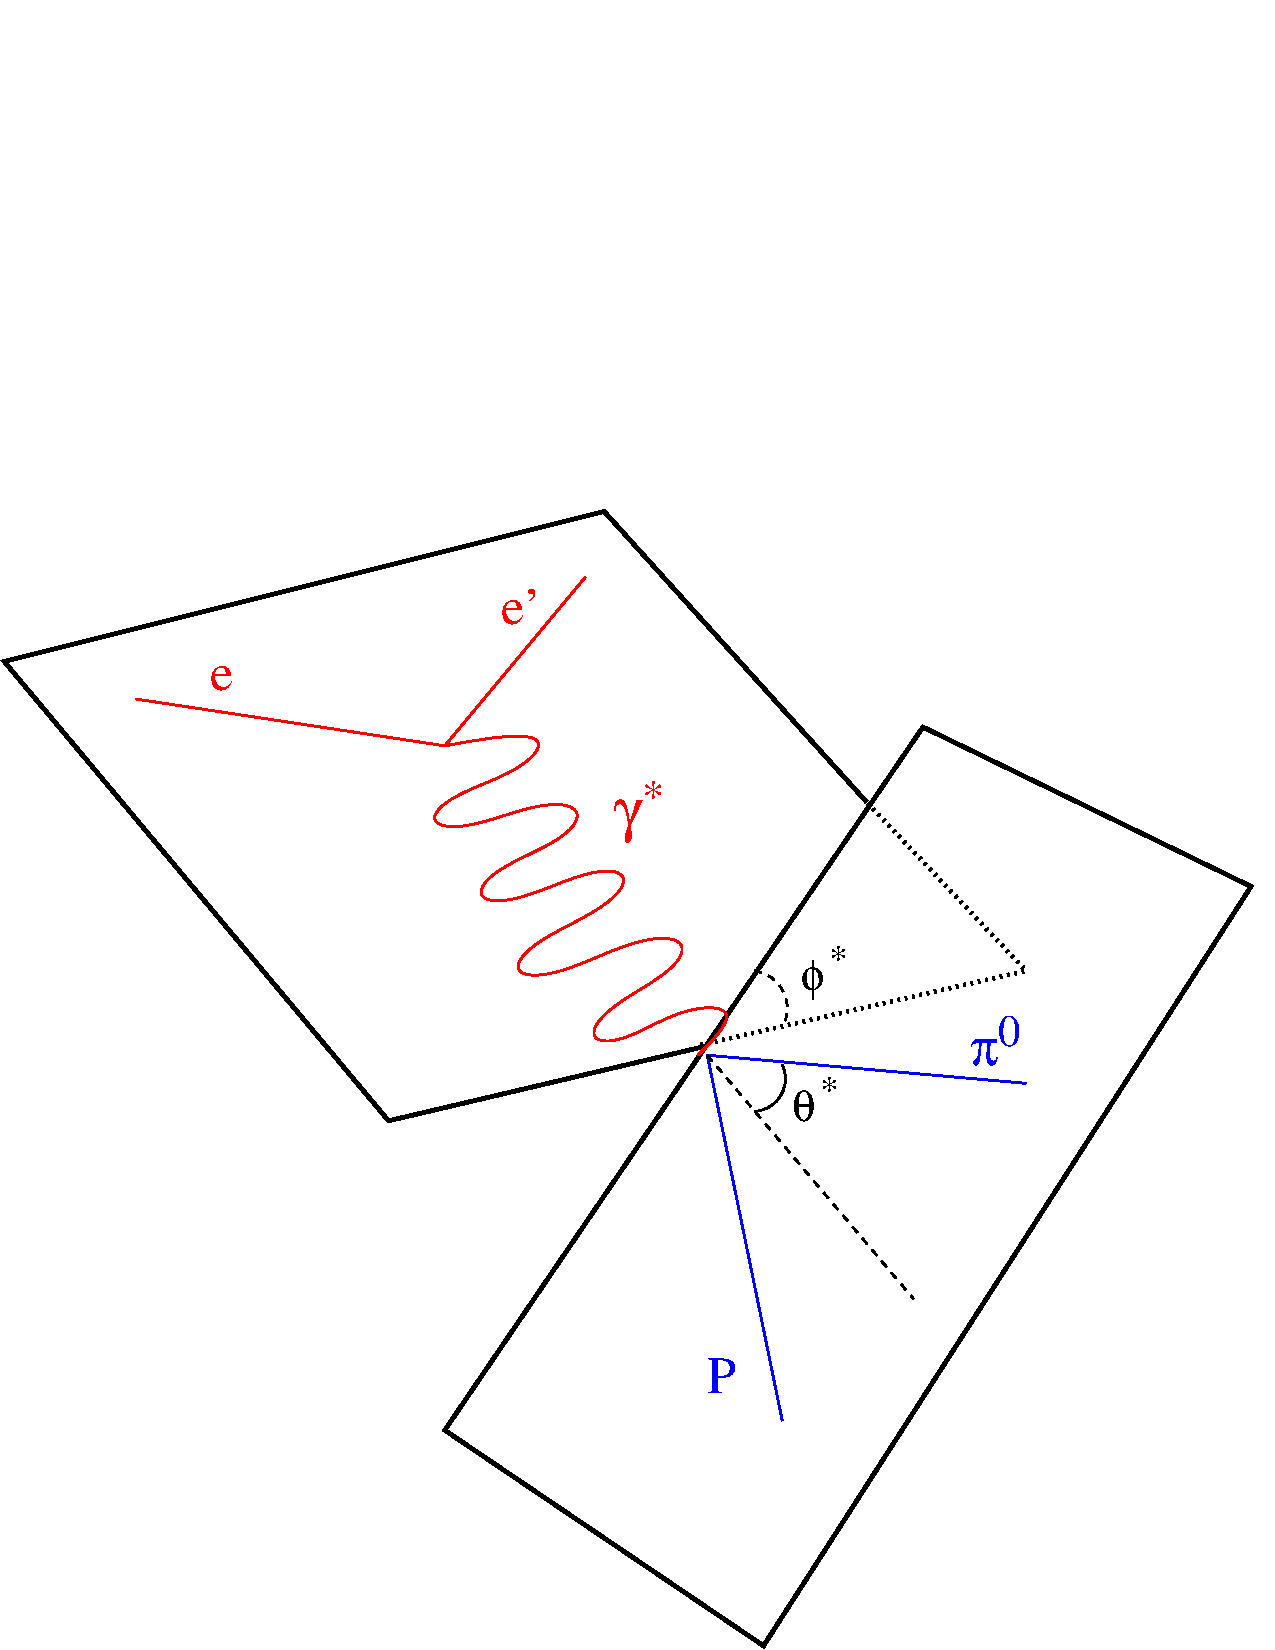
\includegraphics[width = 7cm, bb = 0 -50 570 580]{systematics/img/kine}
  \caption[Schematics of  $\pi^0$ electroproduction]
          { Schematics of  $\pi^0$ electroproduction. The $z-axis$
           is oriented along the beam line (incoming $e$) . On the right the definitions
           of the angles $\phi^*$ and $\theta^*$.}
  \label{fig:kinema}
 \end{center}
\end{figure} 




\subsection{The Invariant Method}
The calculation of $\theta^*$ with the invariant method is based on the identity $p_z = |\vec{p}|\cos\theta$.
While $p_z$ is calculated using the Lorentz method described above, $|\vec{p}|$ is derived using electron
kinematics and the assumption of $\Delta \rightarrow p,\pi^0$ decay using the two body decay in the c.m.
formula:
$$
 p = \Dfrac{\sqrt{ [W^2-(m_p-m_{\pi^0})^2][(W^2-(m_p+m_{\pi^0})^2 ] }}{2}
$$


\subsection{Comparison}\label{sec:cmsystcomp} 
In order to study the above methodologies, a Monte Carlo simulation was used. Furthermore, the
data  were fitted  using both methods.

An example of the simulation result is illustrated in \F{fig:cmctheta}, where the $\cos\theta^*$ distribution 
is plotted for generated, "lorentz" and "invariant" events (meaning, events where $\cos\theta^*$ was
calculated using the Lorentz and Invariant method respectively). The histos are normalized for a better comparison.
When calculating the c.m. angle for the generated events, the original $\pi^0$ four vector was used, since it was kept in the datastream.
For the Lorentz and Invariant case, the scattered electron and proton four vectors were used instead, as during the data analysis.
Hereafter, {the \color{blue}Lorentz} method events will be plotted in blue, while the  {the \color{red}Invariant} method ones
will be plotted in red.

\F{fig:cmctheta} a) shows the three methods for the generated events (before they are processed with GSIM).
The differences between the distributions are due to the radiation of the electron arm (see \F{fig:rad}). In 
\F{fig:cmctheta} b) the same quantities are plotted after the fiducial cuts are applied (and still before GSIM).
A slight distortion is seen. At forward angles, the Lorentz method is closer to the generated $\pi^0$ angle.
In \F{fig:cmctheta} c) the distributions after GSIM and software reconstruction. 
Both at backward and forward angle, the Lorentz method is closer to the generated $\pi^0$ angle.
The Invariant method shows some unphysical $\cos\theta^* > 1$ events. These are due 
to the smearing introduced by the CLAS detectors and reconstruction software and possibly 
to the rescattering of the proton in the torus coils. While the calculation of $|\vec{p}|$ is based on
the assumption of $\Delta \rightarrow p,\pi^0$ decay and uses only the electron kinematics, the calculus
of $p_z$ is not and this can lead to events where $p_z > |\vec{p}|$.
In the Lorentz method, $\cos\theta^*$ is calculated from the four vector components of $x_\mu^{CM}$ so by
definition its limits are $-1,1$. 



The events with $\cos\theta^* > 1$
for the invariant method are dealt in three ways, all included in the analysis: 
1) They are rejected. 2) A cut at $\cos\theta^* < 1.05$ is introduced
to recover the "smeared" events, but to still reject possible rescattering from the coils. In this case, the events with
$1 < \cos\theta^* < 1.05$ are inserted in the last $\cos\theta^*$ bin. 3) They are all inserted in the last $\cos\theta^*$ bin. 
See App. \ref{sec:costhetaplots} for the same plots at different $Q^2$.
\begin{figure}[h]
 \begin{center}
  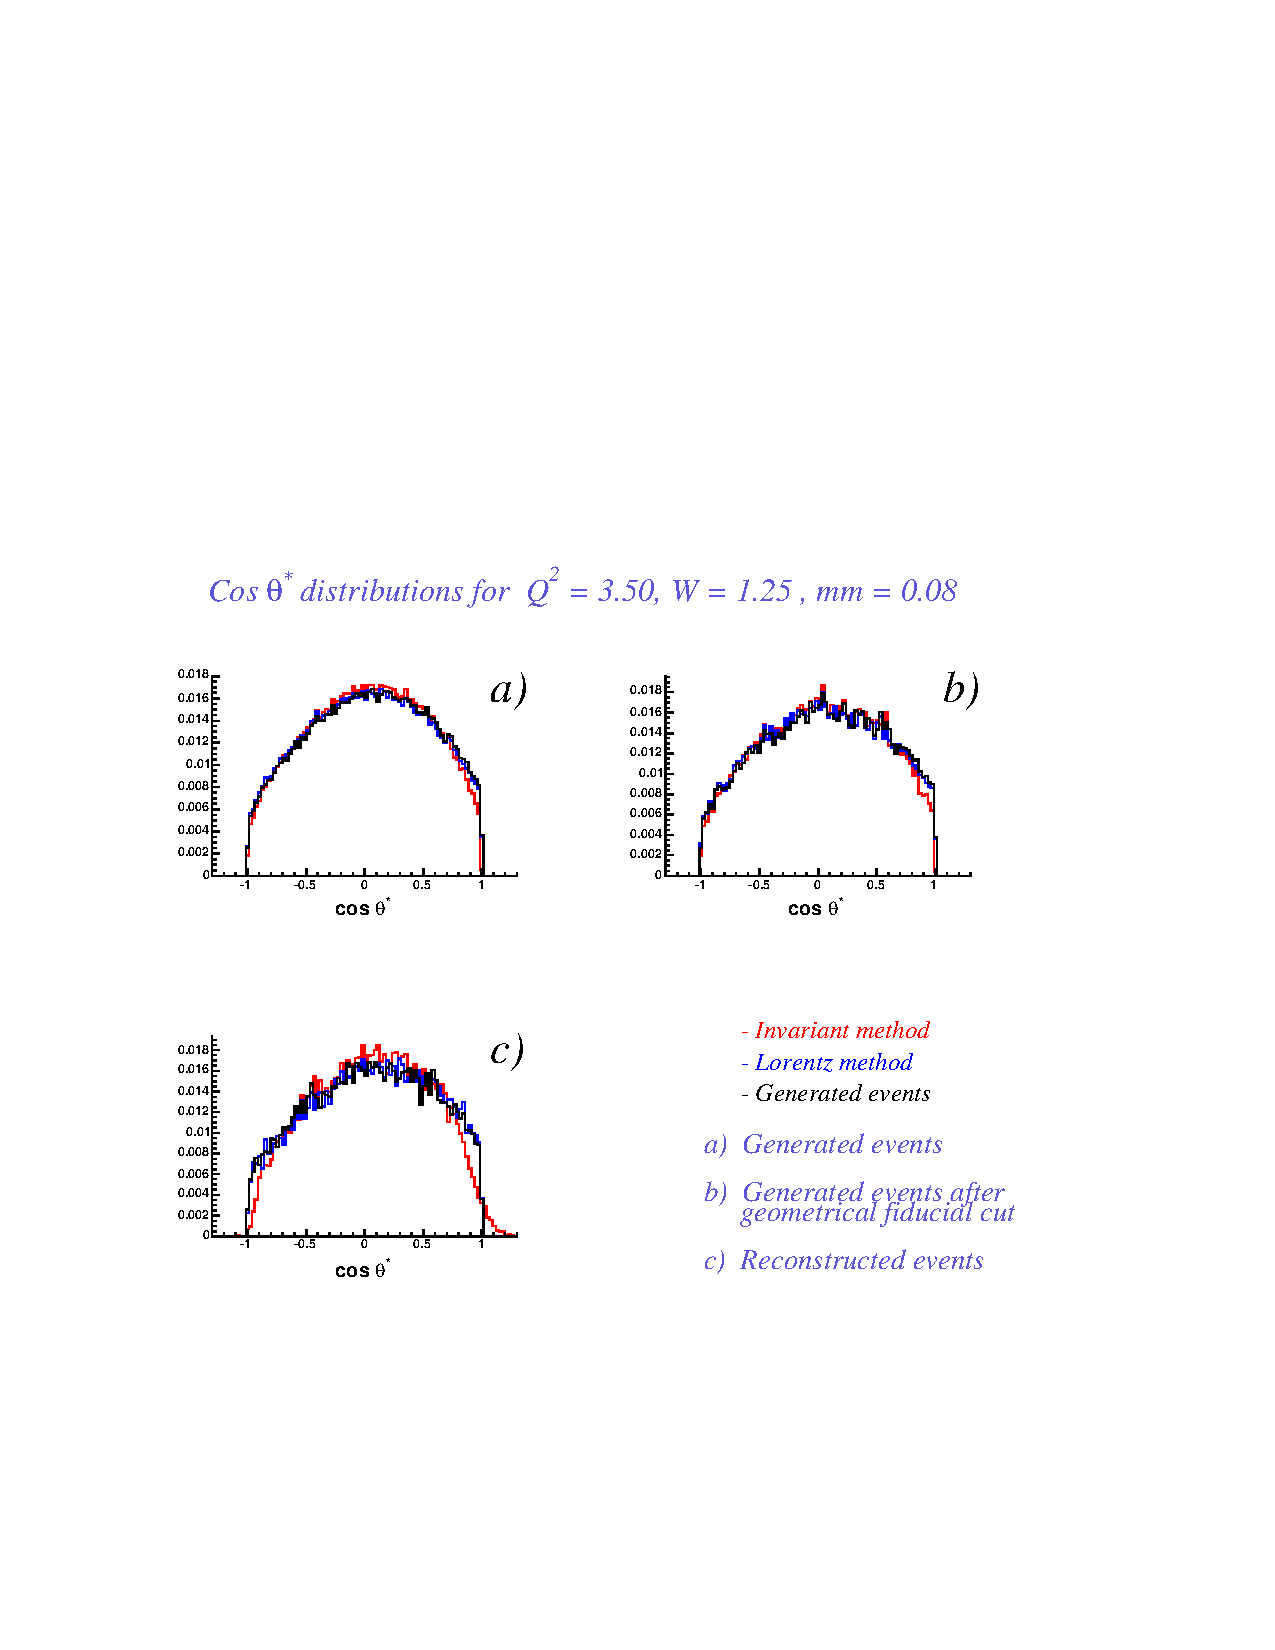
\includegraphics[width = 12cm, bb = 60 140 540 540]{systematics/img/ctheta_q23.50_W1.25_mm0.08}
  \caption{Generated, Lorentz and Invariant reconstructed $cos\theta^*$ distribution for $Q^2=3.5$ $GeV^2$.
           All histograms are normalized to 1.}
  \label{fig:cmctheta}
 \end{center}
\end{figure}  \\
In \F{fig:cmthetaacc} the acceptance is shown for the same $(W,Q^2)$ bin of \F{fig:cmctheta}. The differences
peak at the $\cos\theta^*$ extremes.
\begin{figure}[t]
 \begin{center}
  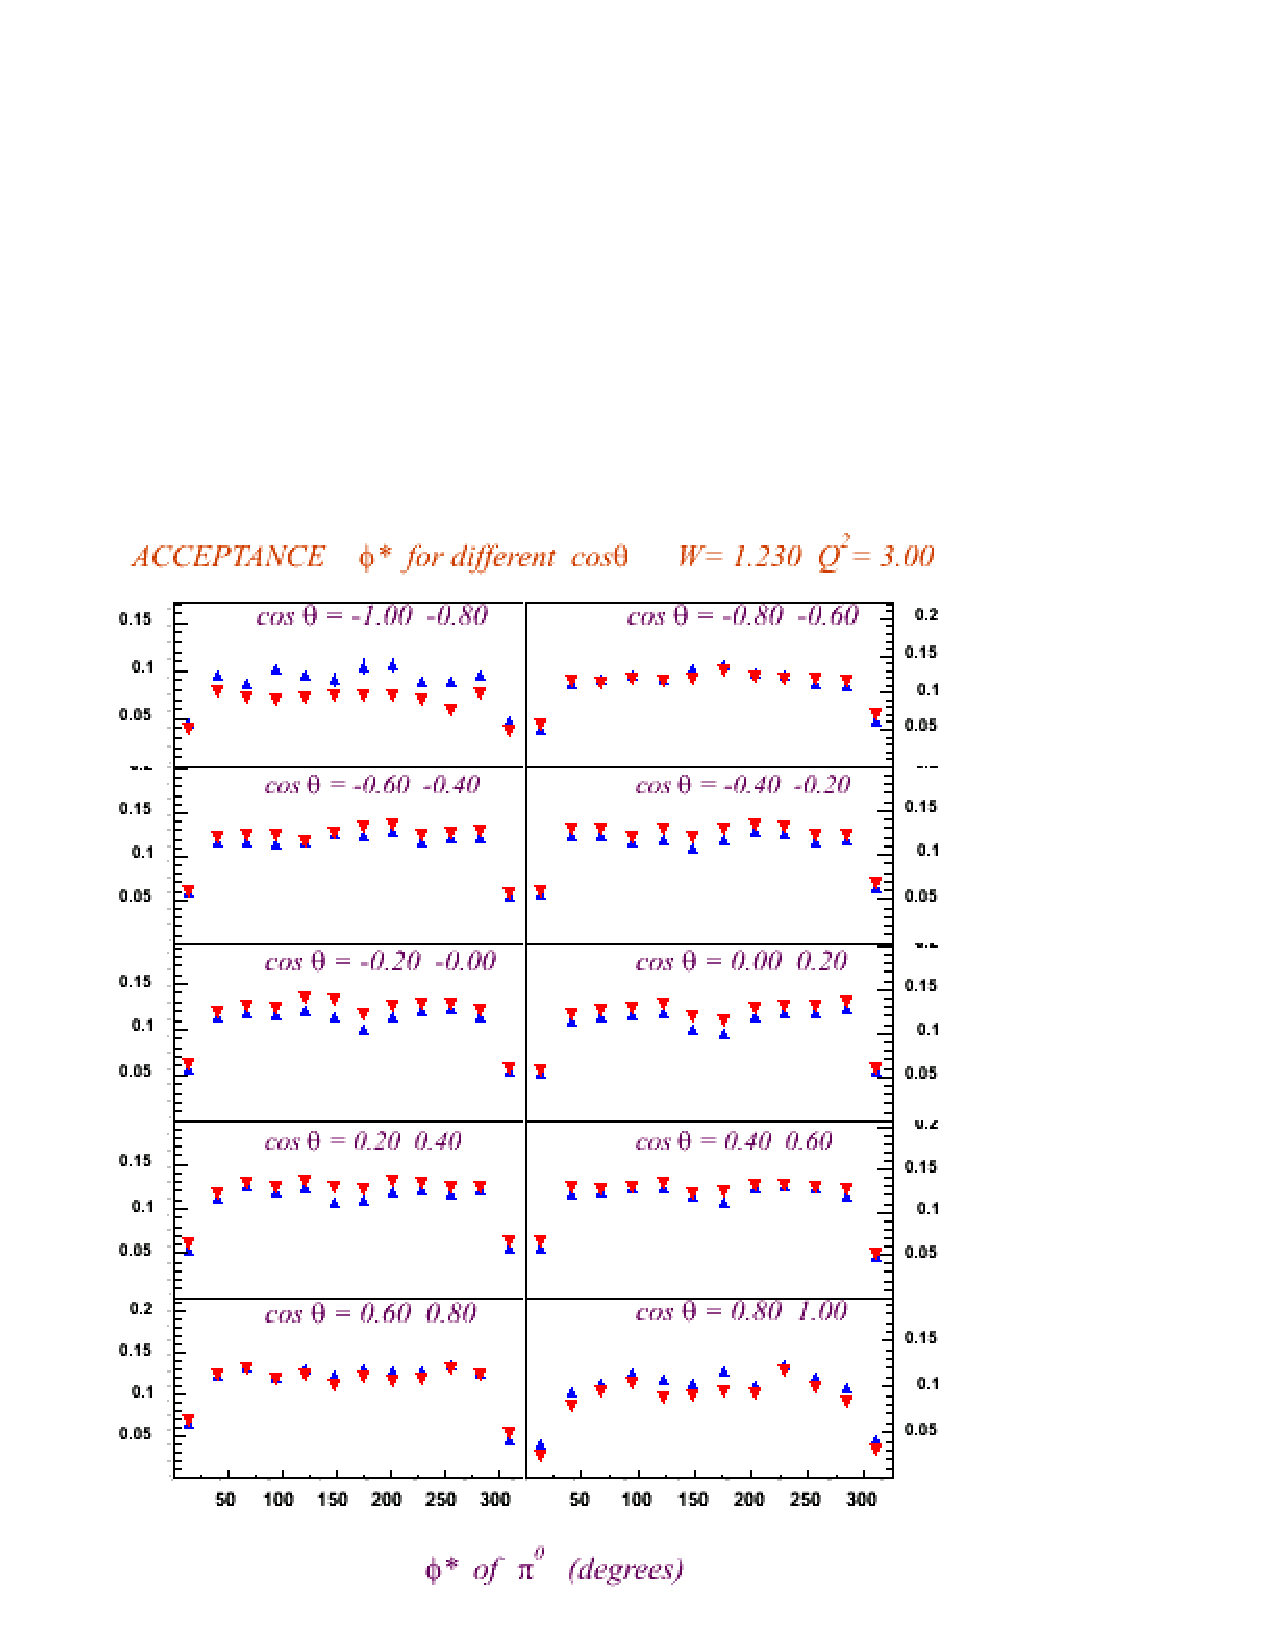
\includegraphics[width = 12cm, bb = 0 20 480 540]{systematics/img/acc_phi_W1.23_Q23.00_mm0.080_ct0.95}
  \caption{Acceptance for $W=1.23$ $GeV$ and $Q^2=3.0$ $GeV^2$. Blue: Lorentz method. Red: Invariant method.
 The differences of the two methodes are maximum at the extremes $\cos\theta^*$ , especially at $\cos\theta^*=-0.9$}
  \label{fig:cmthetaacc}
 \end{center}
\end{figure} 
The c.m. differential cross section is shown in \F{fig:cmthetacro}. When performing the $a+b\cos\phi^*+c\cos 2\phi^*$ fit
and extracting the structure functions, such small difference at extremes $\cos\theta^*$  play an important rule. The 
curvature of $\sigma_T + \epsilon\sigma_L$ at the $\Delta$ pole is most sensitive to the electric quadrupole amplitude 
$E_{1+}$.
Differences of the $\sigma_T + \epsilon\sigma_L$ are illustrated in \F{fig:cmthetalpt}. During the analysis, the structure functions
were expanded in Legendre polynomials. The coefficients of the $\sigma_T + \epsilon\sigma_L$ expansions for the two methods
are illustrated in \F{fig:cmthetalpt}. The $A_2$ coefficient (which is basically the curvature of $\sigma_T + \epsilon\sigma_L$), 
differs by a factor of two. A non zero value of the $A_3$, $A_4$ coefficients would be the signal of 
$\ell>1$ components of the $(\pi^0,p)$ orbital angular momentum. \\
During the multipole truncation analysis,
the $M_{1+}$ dominance is assumed and the ratios $E_{1+}/M_{1+}$ and $S_{1+}/M_{1+}$
are calculated. Both the cases $\ell \le 1$ and $\ell \le 2$ are considered. 
An example of this extraction is shown in \F{fig:cmthetares}.

\begin{figure}[h]
 \begin{center}
  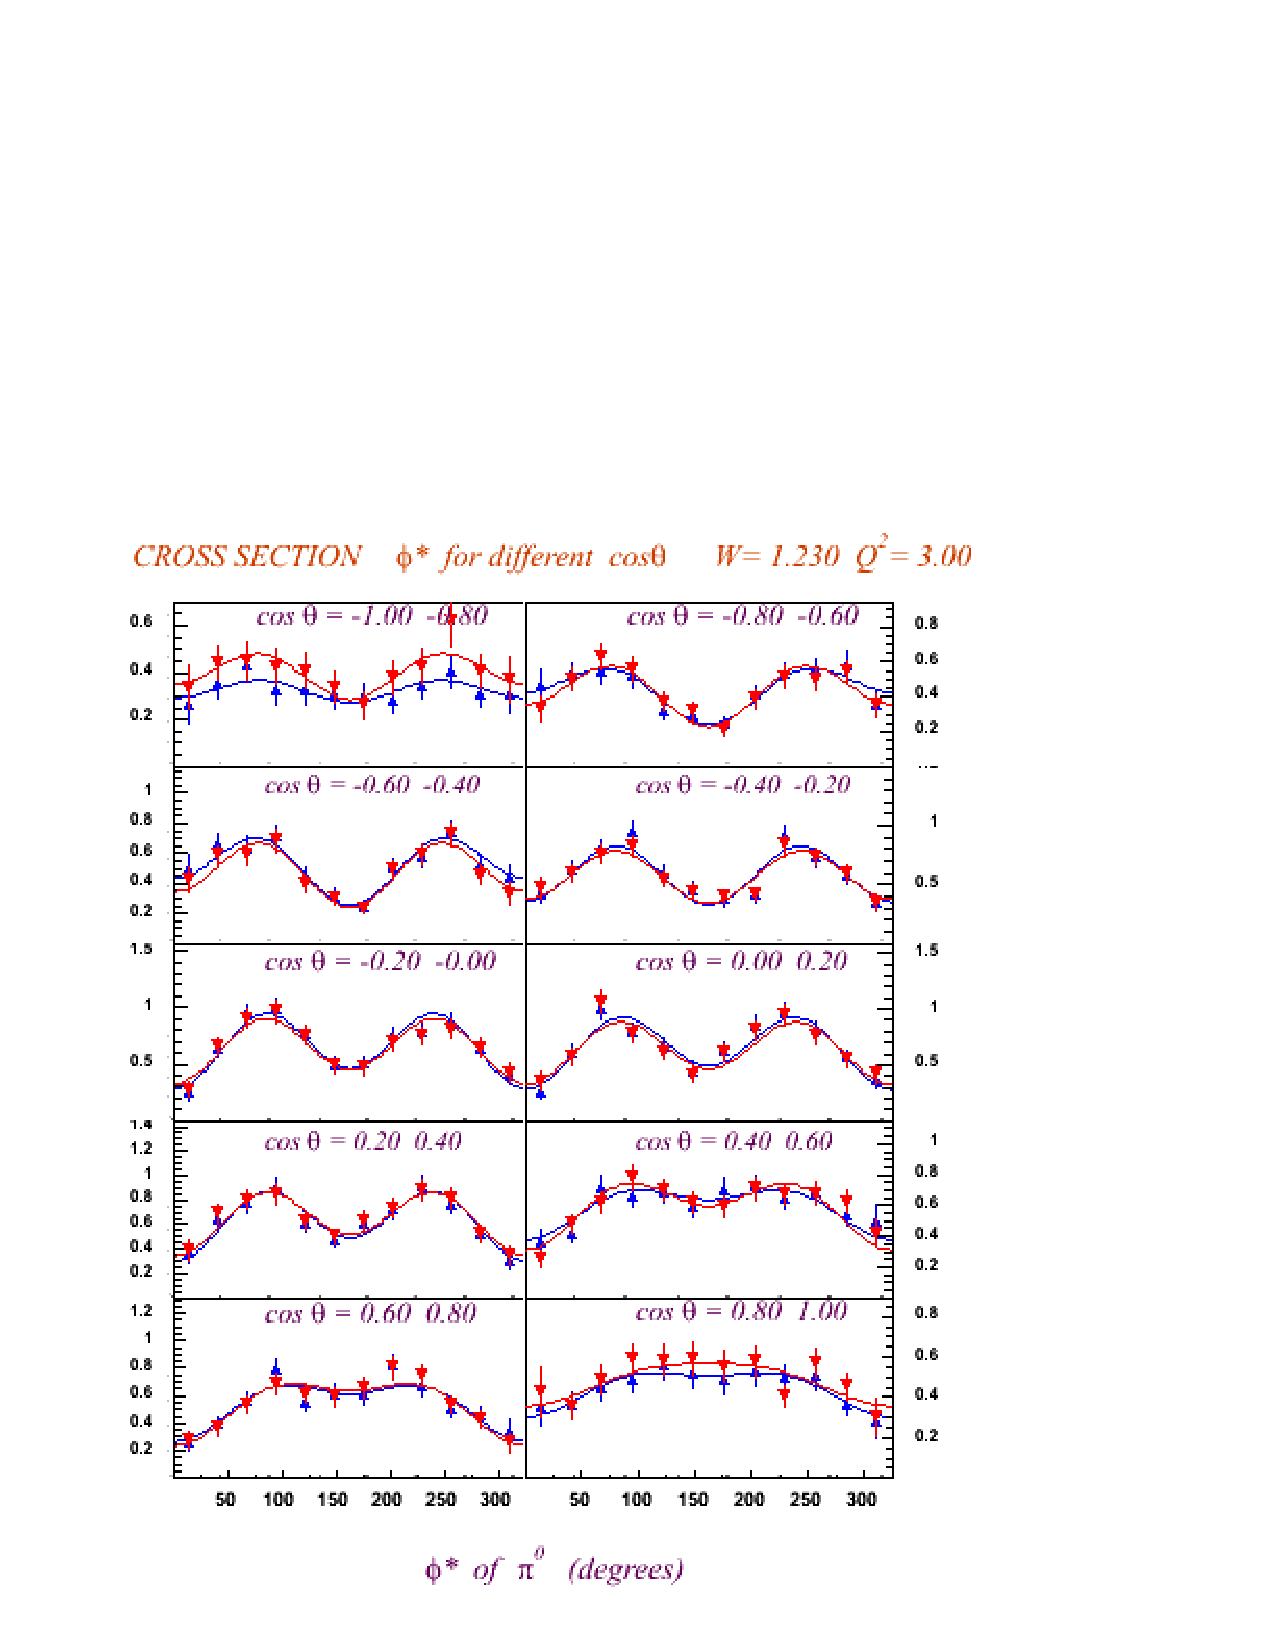
\includegraphics[width = 12cm, bb = 0 20 480 540]{systematics/img/cro_phi_W1.23_Q23.00_mm0.080_ct0.95}
  \caption{C.m. cross section for $W=1.23$ $GeV$ and $Q^2=3.0$ $GeV^2$. Blue: Lorentz method. Red: Invariant method.
           the two methods are similar except at the $\cos\theta^*$ extremes. }
  \label{fig:cmthetacro}
 \end{center}
\end{figure} 
\begin{figure}[h]
 \begin{center}
  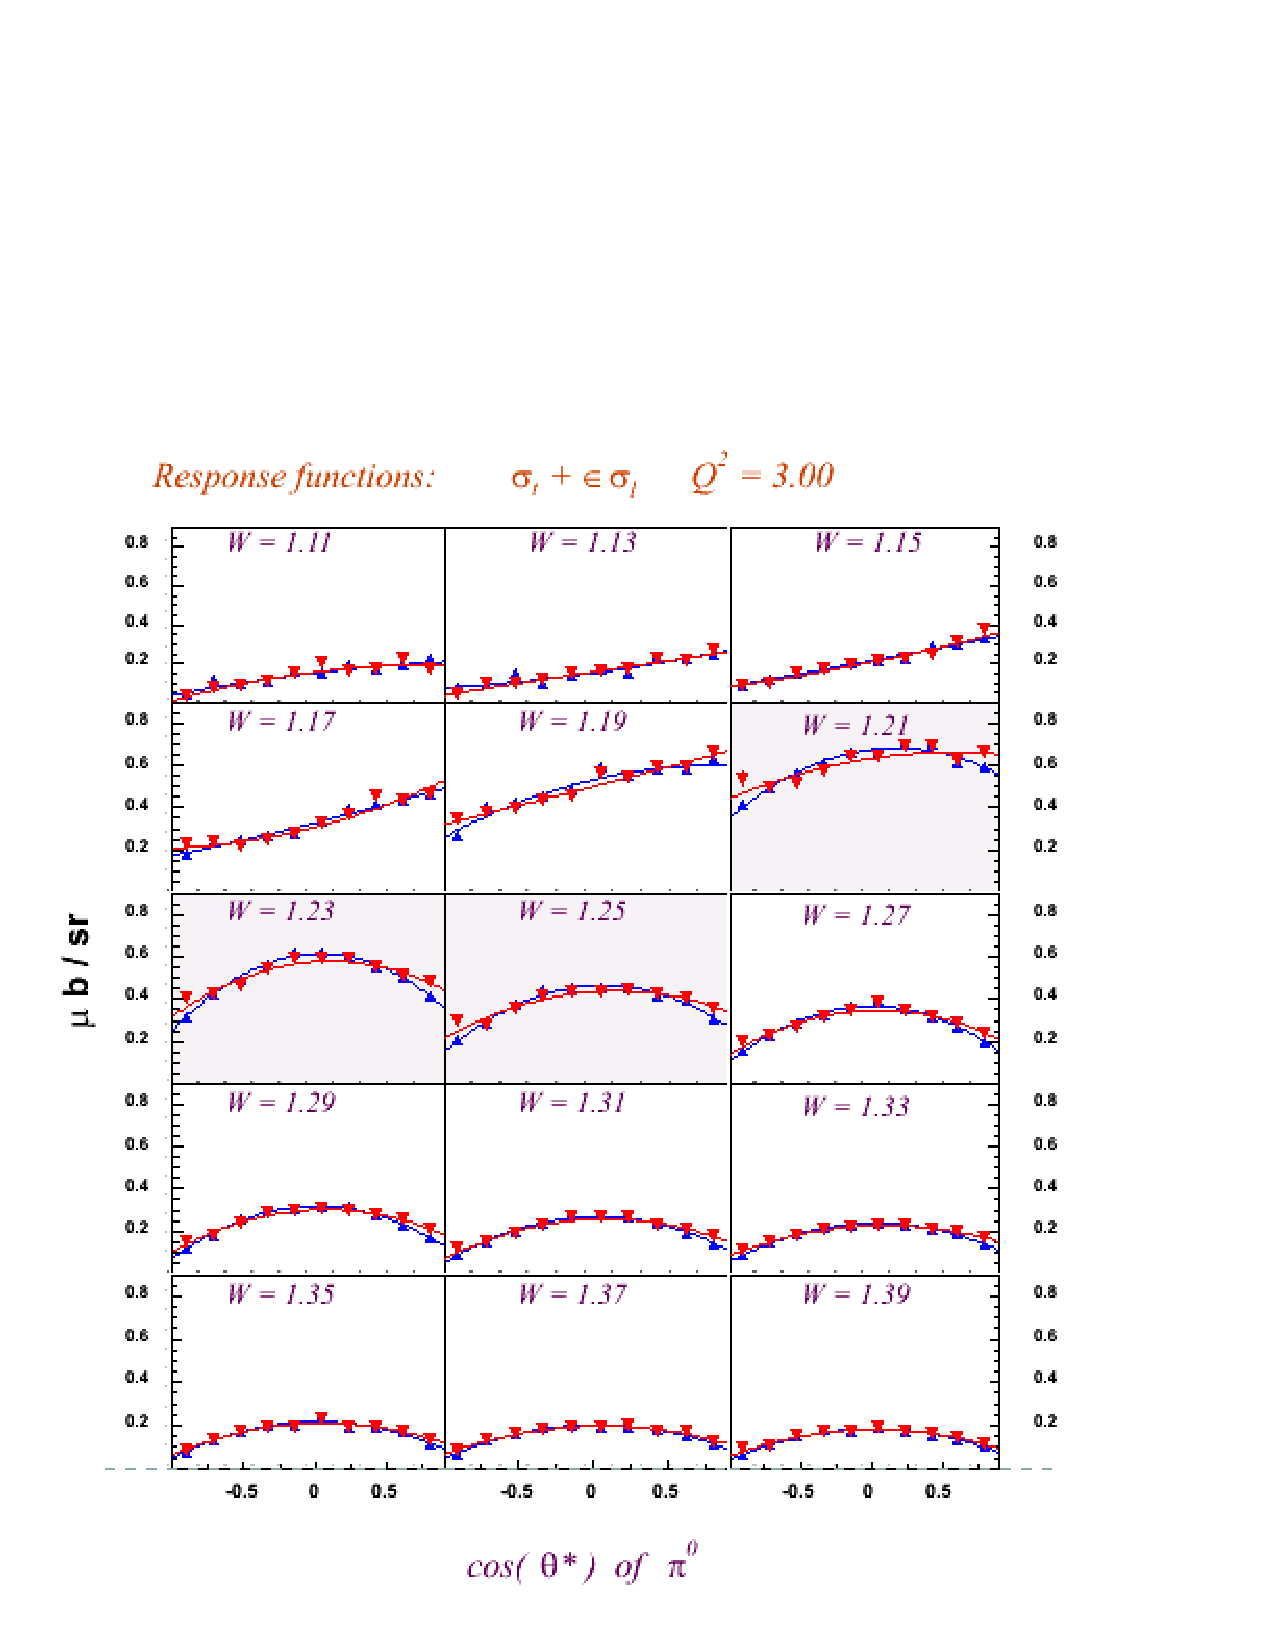
\includegraphics[width = 12cm, bb = 40 20 580 580]{systematics/img/lpt_Q23.00_mm0.080_ct0.95_L1}
  \caption{$\sigma_T + \epsilon\sigma_L$ for $Q^2=3.0$ $GeV^2$. Blue: Lorentz method. Red: Invariant method.
           Note that the curvature of $\sigma_T + 
           \epsilon\sigma_L$ at the $\Delta$ pole determines the amplitude of the electric 
            quadrupole $E_{1+}$. See also \F{fig:cmthetaacoeff}}
  \label{fig:cmthetalpt}
 \end{center}
\end{figure} 
\begin{figure}[h]
 \begin{center}
  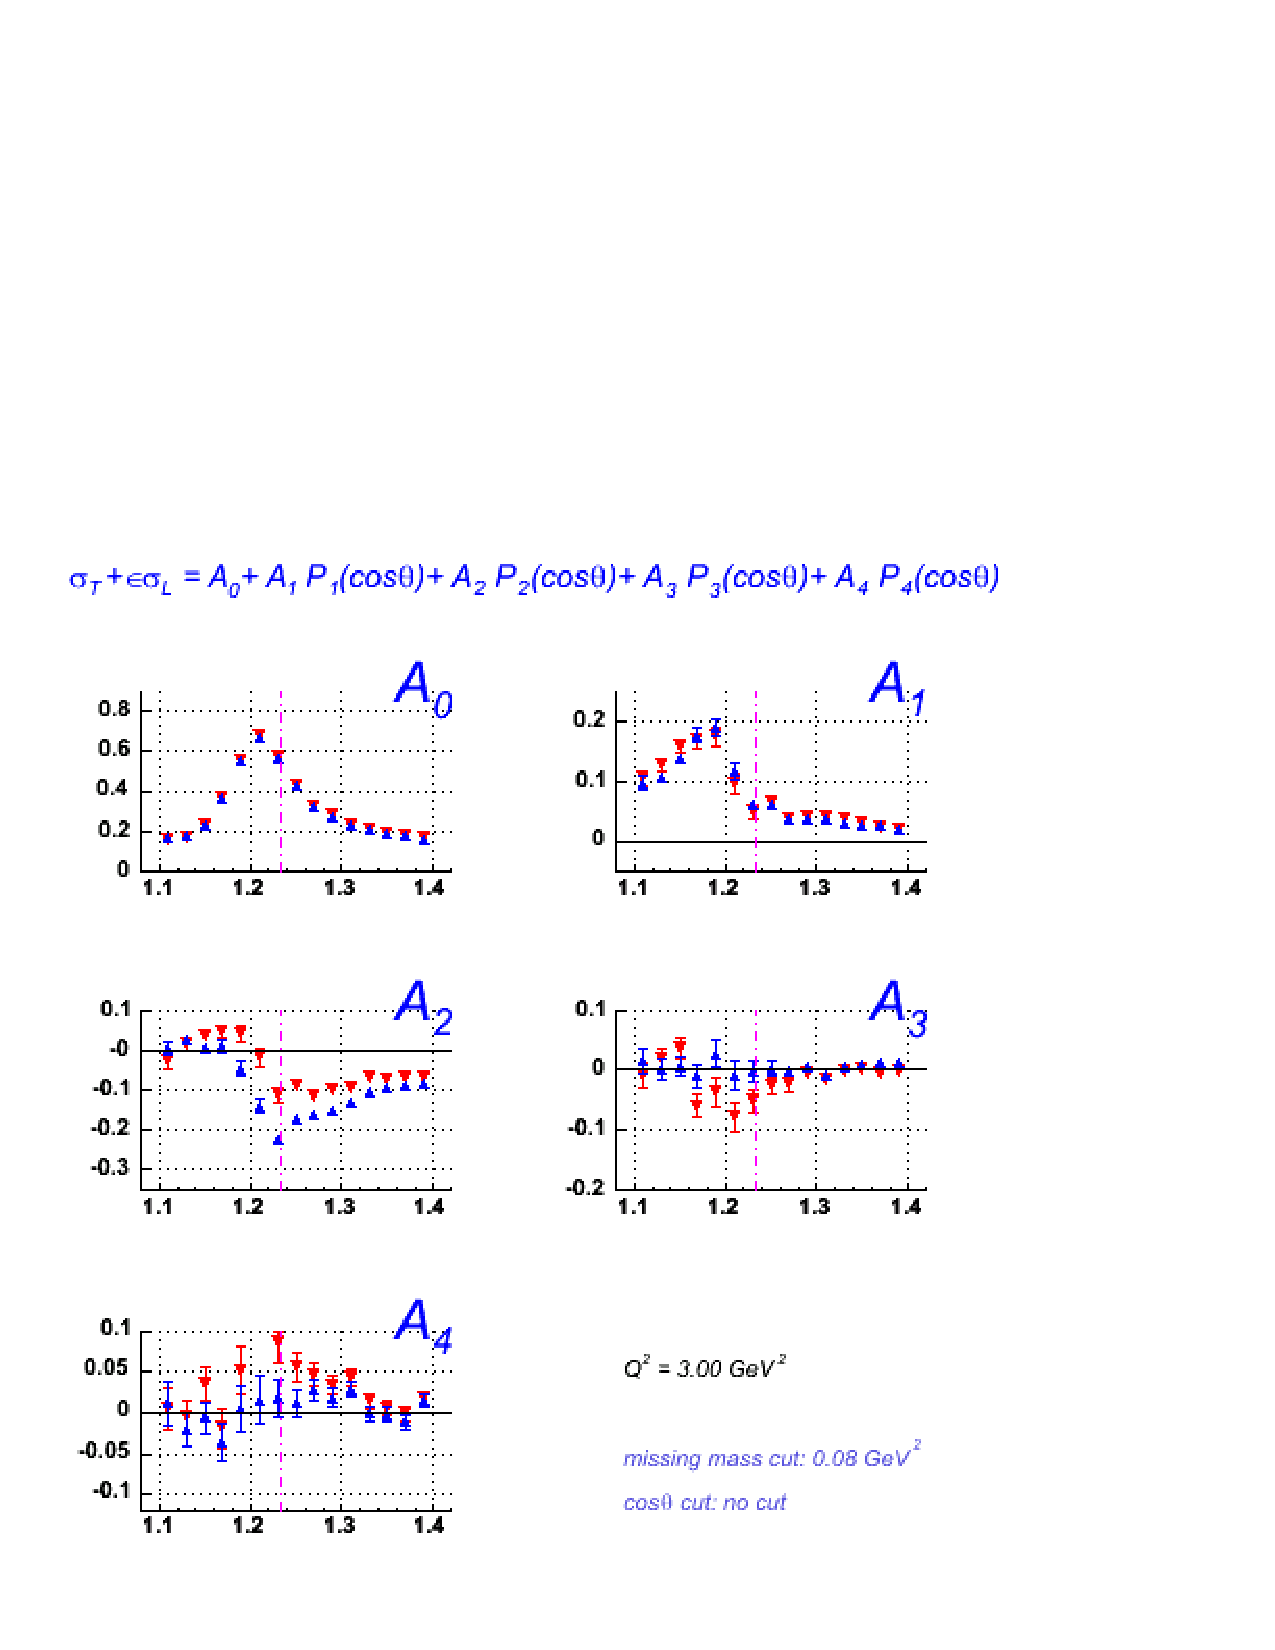
\includegraphics[width = 12cm, bb = 0 20 480 540]{systematics/img/A_coeff_q23.00_mm0.080_ct100.00_L2}
  \caption{The coefficients of the $\sigma_T + \epsilon\sigma_L$ expansions as a function of $W$ 
           for the Invariant and Lorentz method.
           Blue: Lorentz method. Red: Invariant method. The $A_2$ coefficient at the $\Delta$ pole
           differs by a factor of two. A non zero value of the $A_3$, $A_4$ coefficients would be the signal of 
            $\ell>1$ components of the $(\pi^0,p)$ orbital angular momentum.}
  \label{fig:cmthetaacoeff}
 \end{center}
\end{figure} 
\begin{figure}[h]
 \begin{center}
  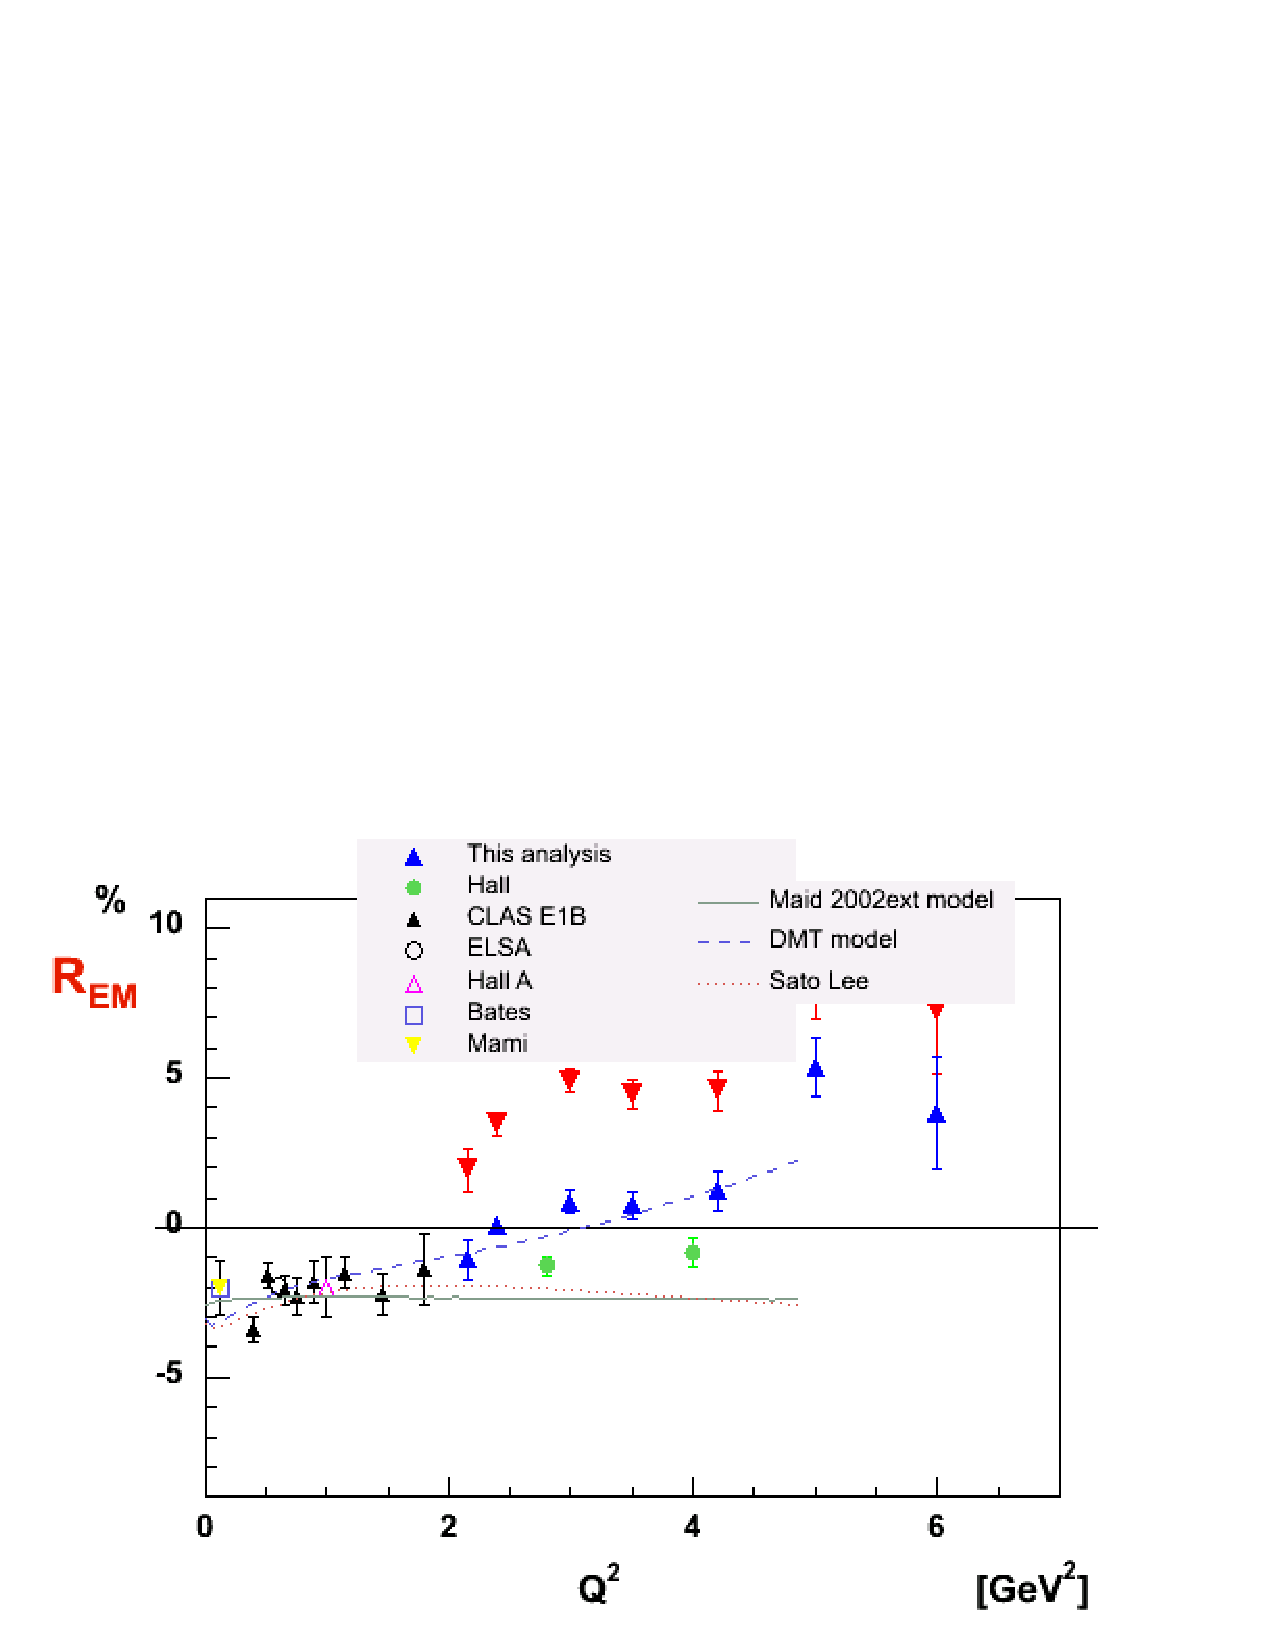
\includegraphics[width = 10cm, bb = 0 0 600 460]{systematics/img/ratios_e1om1_mm0.080_ct0.95_L2}
  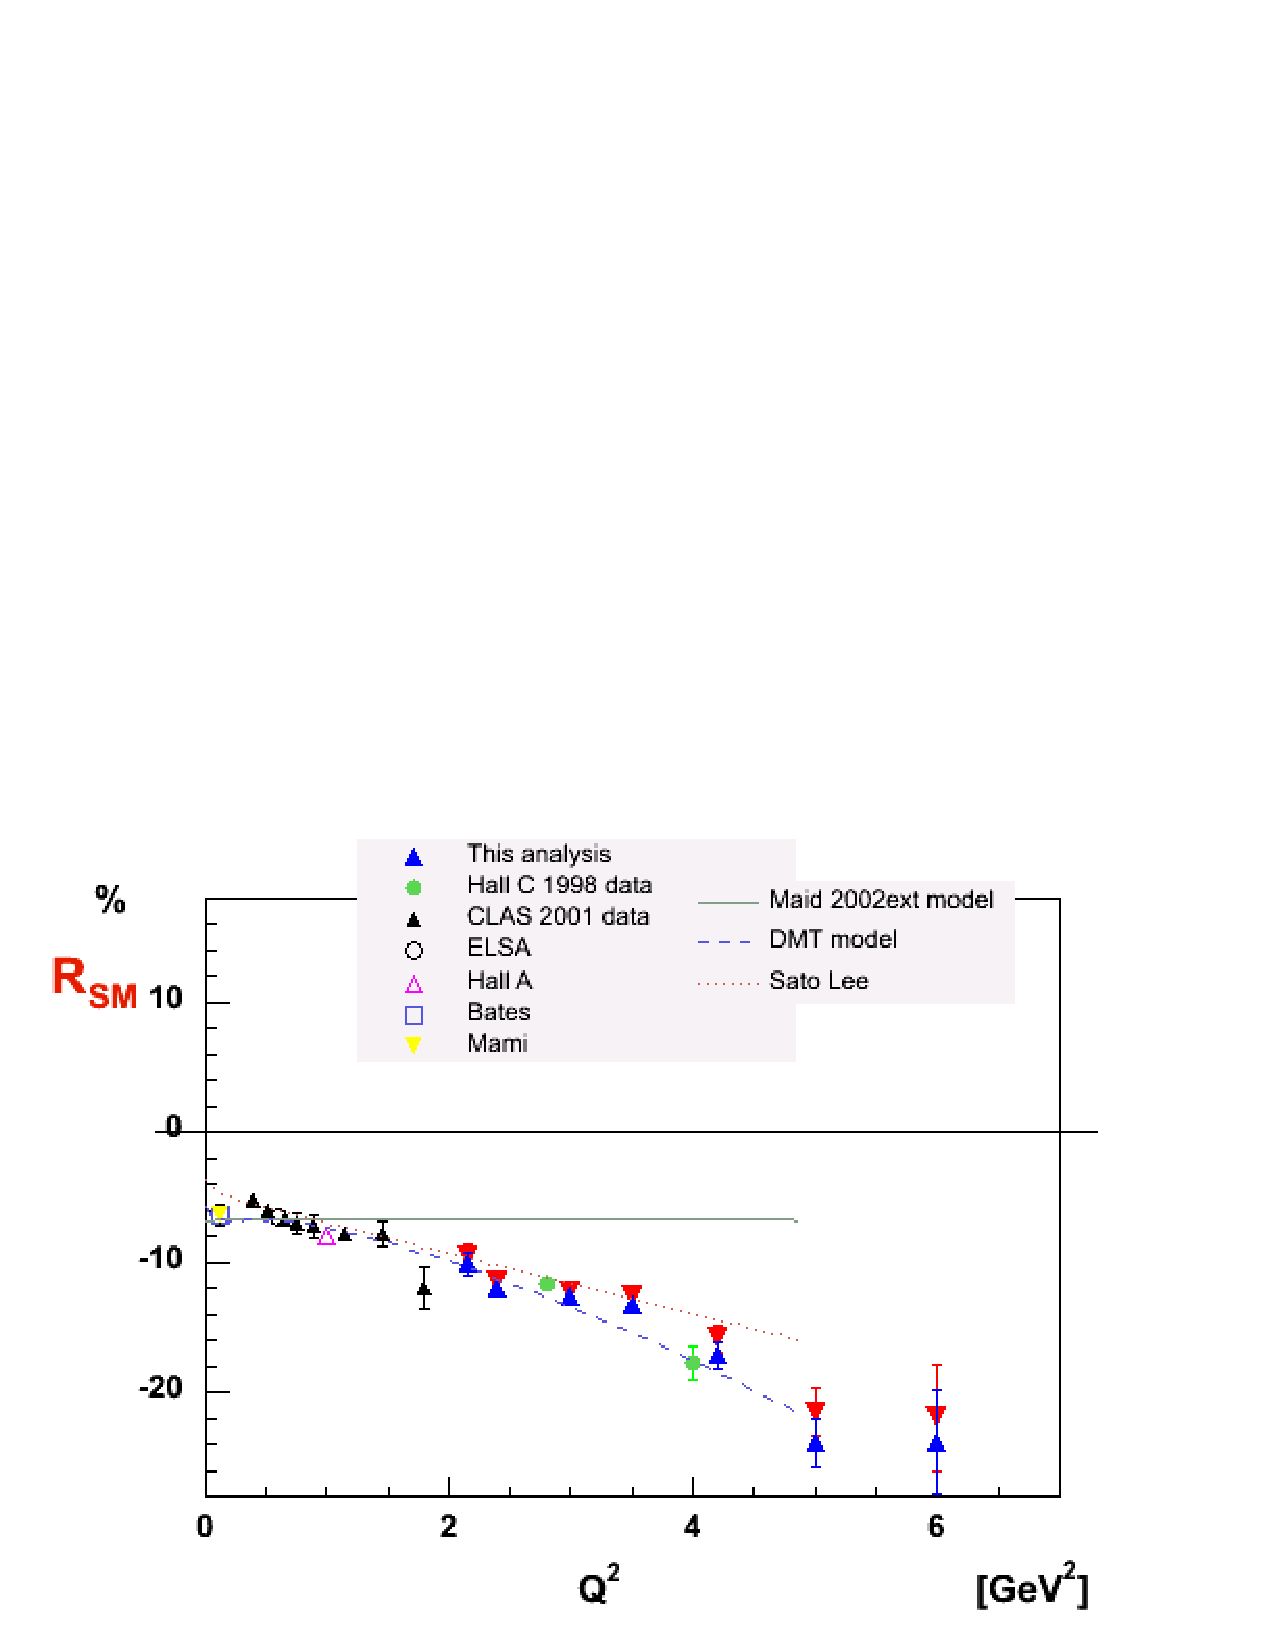
\includegraphics[width = 10cm, bb = 0 0 600 460]{systematics/img/ratios_s1om1_mm0.080_ct0.95_L2}
  \caption{The $E_{1+}/M_{1+}$ and $S_{1+}/M_{1+}$ ratios calculated using the truncated multipole 
           analysis for the Invariant and Lorentz method.
           Blue: Lorentz method. Red: Invariant method. The big discrepancy for $E_{1+}/M_{1+}$ is due to the curvature difference of the  
           $\sigma_T + \epsilon\sigma_L$ at the $\Delta$ pole.}
  \label{fig:cmthetares}
 \end{center}
\end{figure} 

\subsection{Conclusions}
The Lorentz method better reproduces the generated Monte Carlo $\pi^0$ c.m angle (see \F{fig:cmctheta} and App. \ref{sec:costhetaplots}) 
The discrepancy in calculating the cross section is amplified during the analysis. The invariant method presents unlikely results for 
the orbital angular momentum of the $(\pi^0,p)$ system and for the $E_{1+}/M_{1+}$ ratio (based on continuity from previous measurements).
For this reasons only the Lorentz method will be considered in the analysis. Different cuts at the $\cos\theta^*$ extremes
are performed and included in the systematic errors.
\cia










\cia \vspace{-2cm}
\section{Missing mass cuts}

Background coming from a residual $ep\rightarrow e'p'\gamma $
and from two pion production processes has been taken into account
in the calculation of the systematic errors by varying the missing mass cut according
to Table \ref{tab:missing_mass_cuts}.


\begin{table}[h]
 \begin{center}
  \begin{tabular}{c | c}
    & \\
    min ($GeV^2$)  &  max ($GeV^2$)  \\ 
    & \\
    \hline
    & \\
    -0.05  & 0.08  \\
    -0.04  & 0.075 \\ 
    -0.04  & 0.07  \\
    -0.03  & 0.065 \\
    -0.02  & 0.06  \\
    & \\
    \hline
  \end{tabular}
 \end{center} 
 \caption{ Missing mass cuts}
 \label{tab:missing_mass_cuts}
\end{table}

The cuts are illustrated in \F{fig:mmcuts}.

\begin{figure}[h]
 \begin{center}
  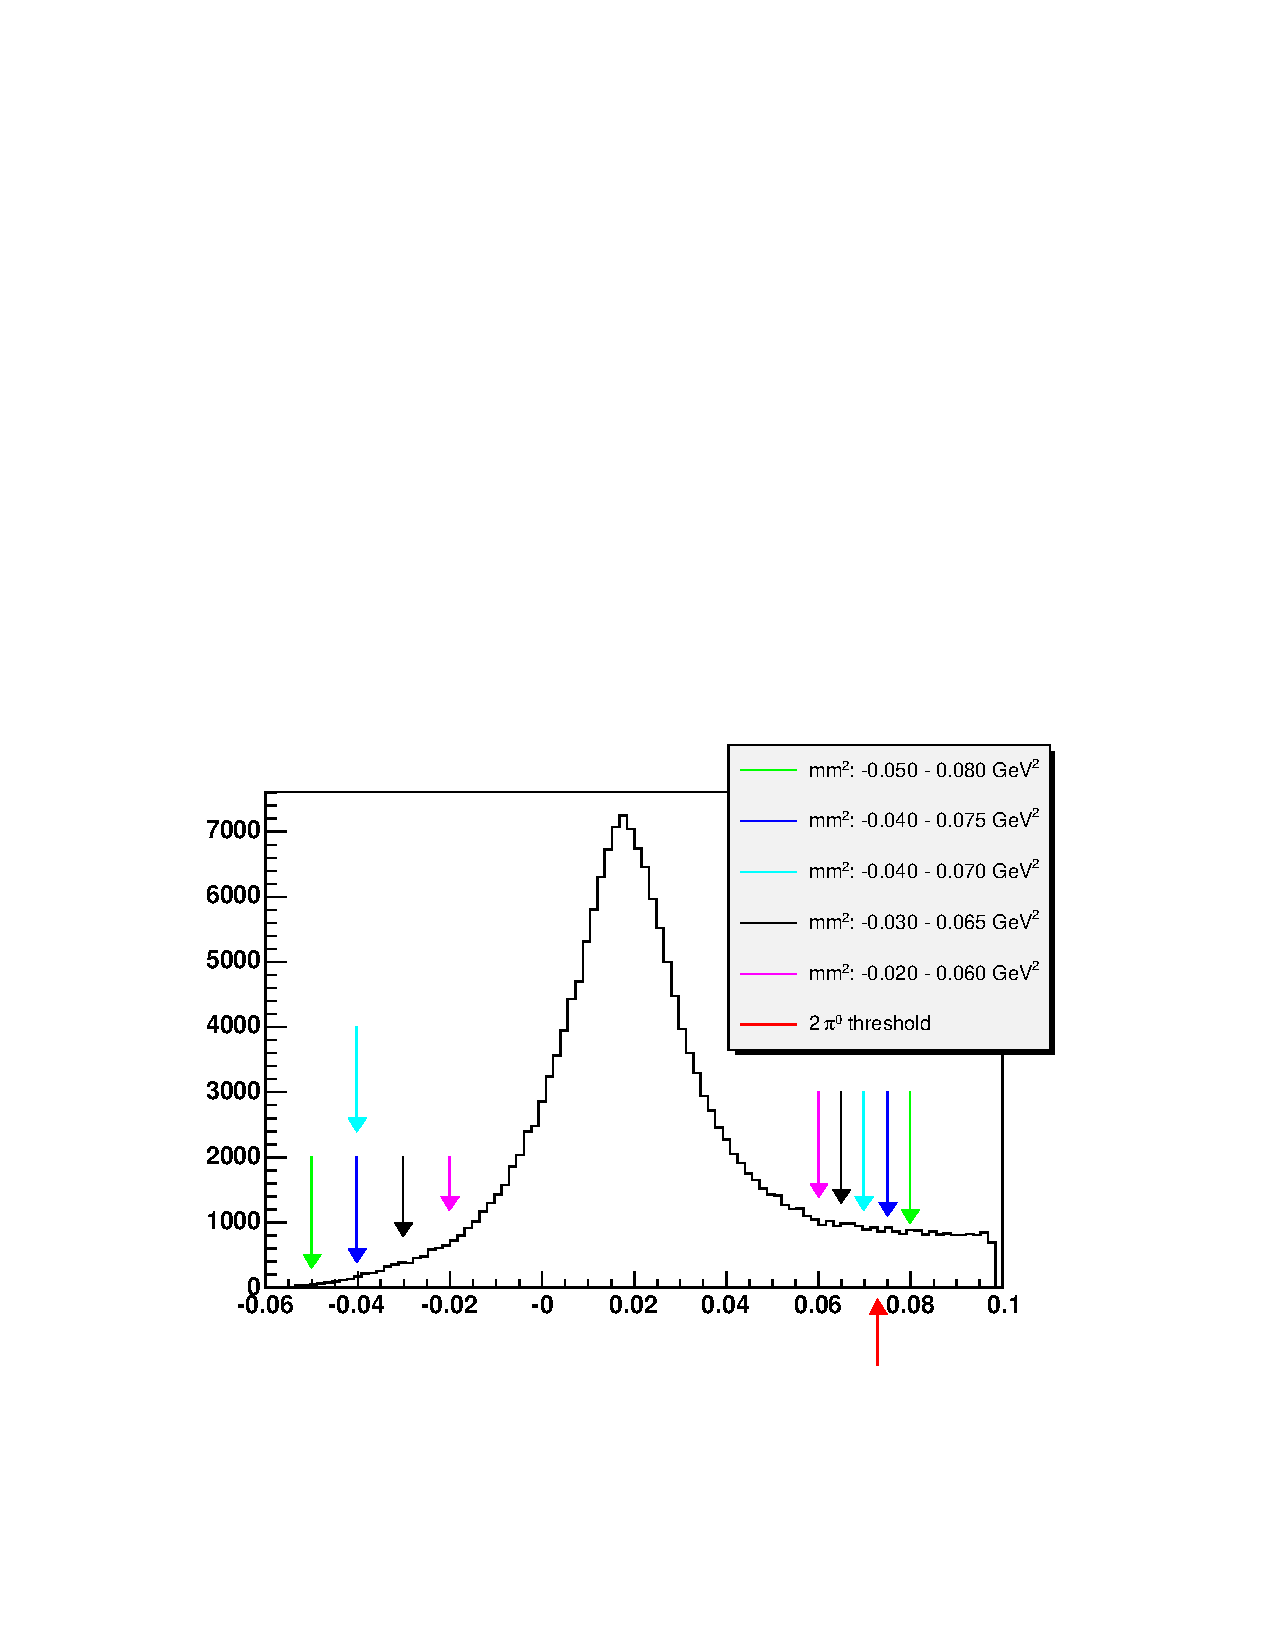
\includegraphics[width = 11cm, bb = 80 140 540 480]{systematics/img/mmcuts}
  \caption{ Missing mass square distribution for $\pi^0$ events and the different
            cuts used for the systematic study. }
  \label{fig:mmcuts}
 \end{center}
\end{figure} 

The variation of the ratios $R_{EM}$ and $R_{SM}$ for the first and last cut is illustrated in 
\F{fig:ratios_mm_syst}.
\begin{figure}[h]
 \begin{center}
  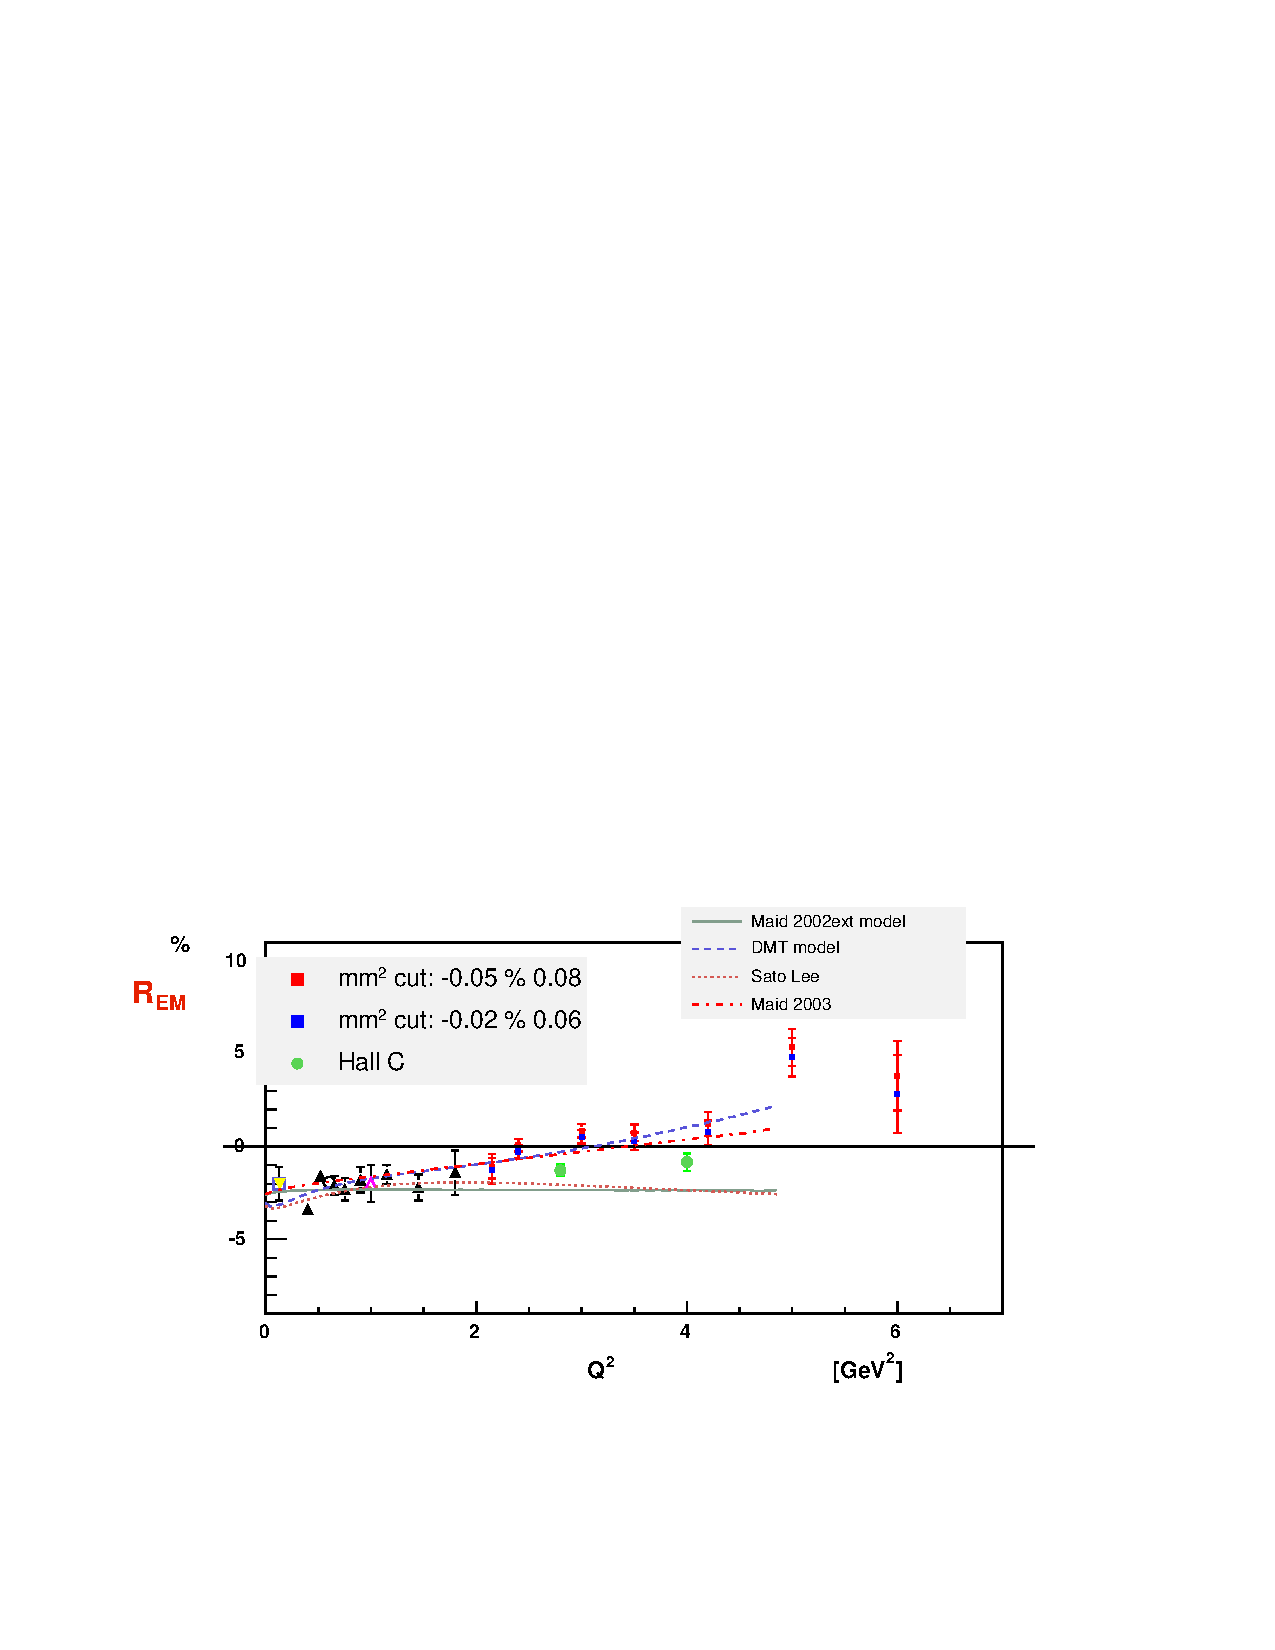
\includegraphics[width = 12cm, bb = 50 120 540 440]{systematics/img/rem_mmsyst}
  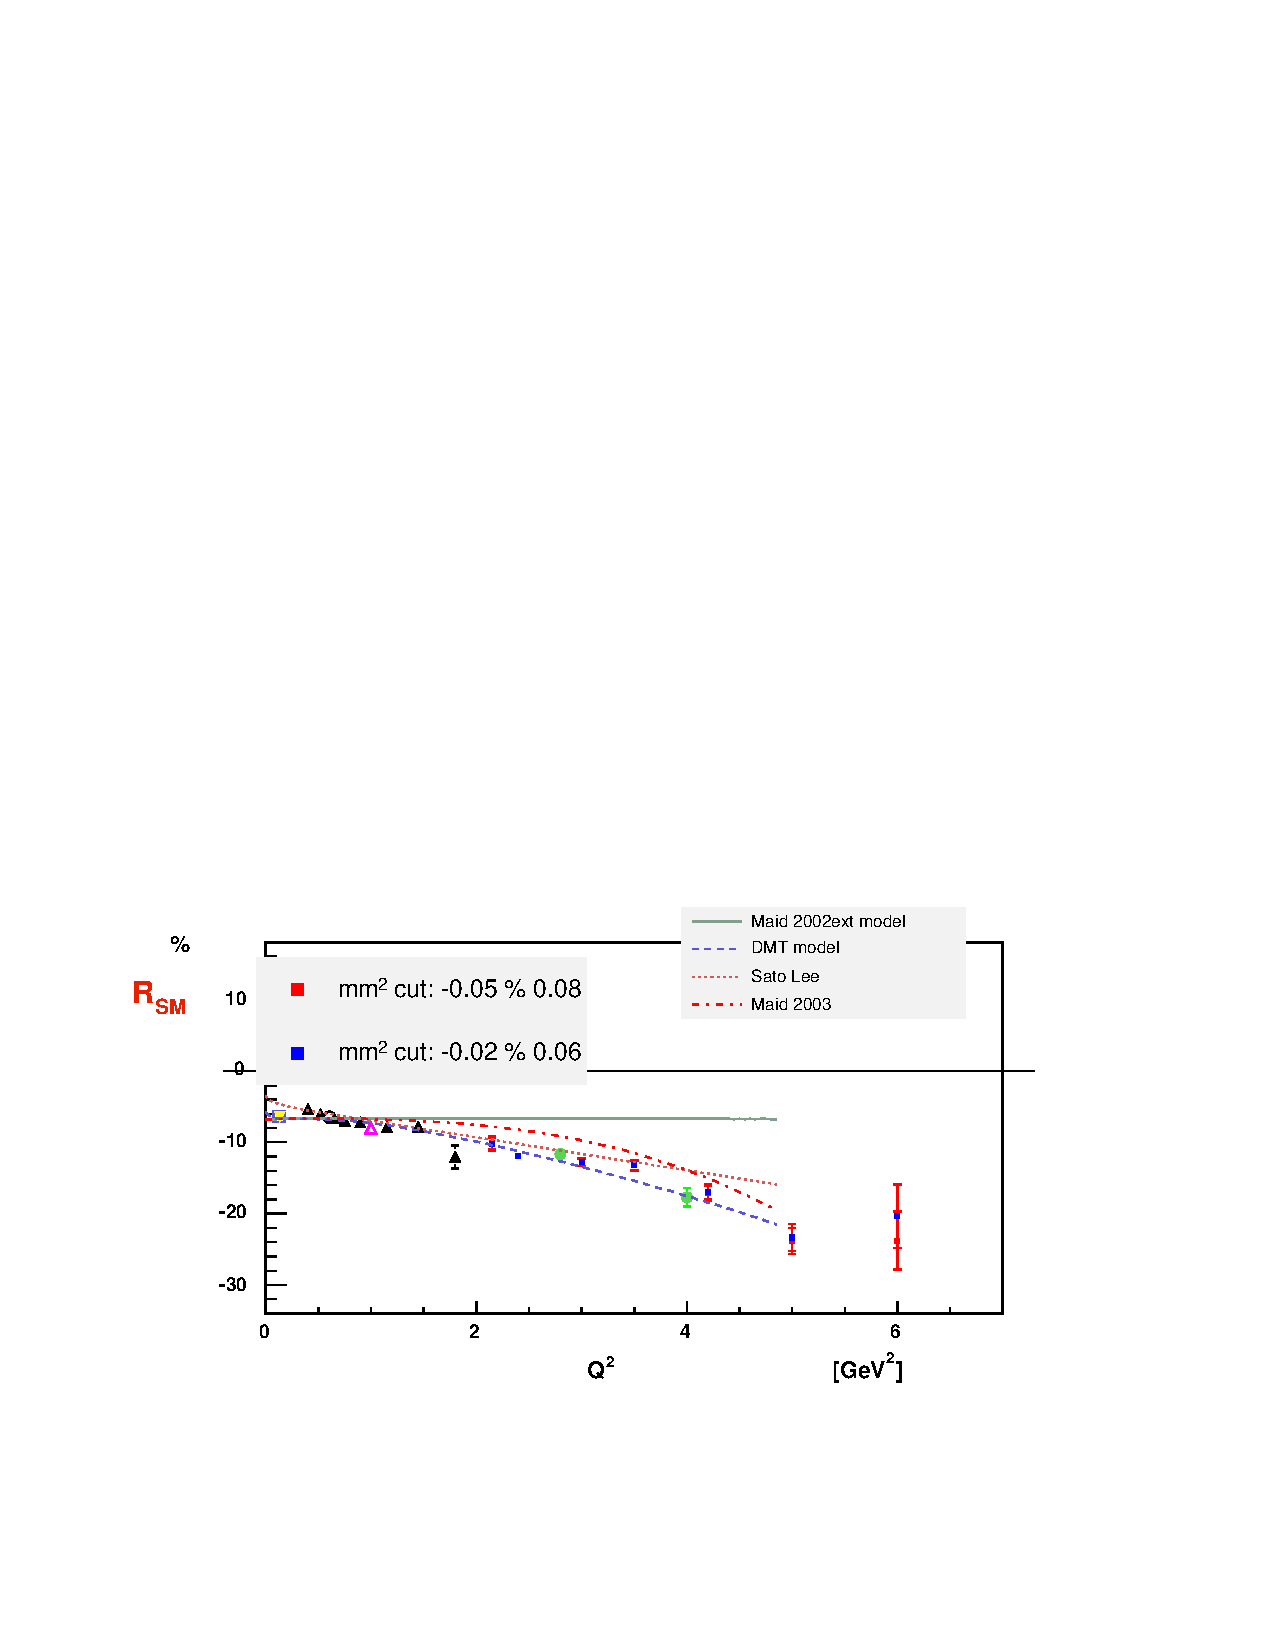
\includegraphics[width = 12cm, bb = 50 100 540 440]{systematics/img/rsm_mmsyst}
  \caption{ Variation of the ratios $R_{EM}$ (top) and $R_{SM}$ (bottom) for the missing mass square cuts:
           $-0.05 < mm^2 < 0.08$ and $-0.02 < mm^2 < 0.06$ }
  \label{fig:ratios_mm_syst}
 \end{center}
\end{figure} 







\cia \vspace{-2cm}
\section{$\cos\theta^*$ cuts}
In Section \ref{sec:cmsystcomp} it was mentioned that the Invariant method of
calculating  $\cos\theta^*$ yelded unphysical results at $\cos\theta^*$ extremes
due to the smearing introduced by the CLAS detectors and reconstruction software and possibly 
to the rescattering of the proton in the torus coils.
In order to study this possible cause of systematic errors, different cuts have been applied
to  $\cos\theta^*$.  The values are shown in  Table \ref{tab:costheta_cuts}.




\begin{table}[h]
 \begin{center}
  \begin{tabular}{c  c}
    & \\
    min &  max   \\ 
    & \\
    \hline
    & \\
    -1     & 1  \\
    -0.95  & 0.95 \\ 
    -0.90  & 0.90  \\
    -0.85  & 0.85 \\
  \end{tabular}
 \end{center} 
 \caption{$\cos\theta^*$  cuts}
 \label{tab:costheta_cuts}
\end{table}


The cuts are illustrated in \F{fig:ccuts}.

\begin{figure}[h]
 \begin{center}
  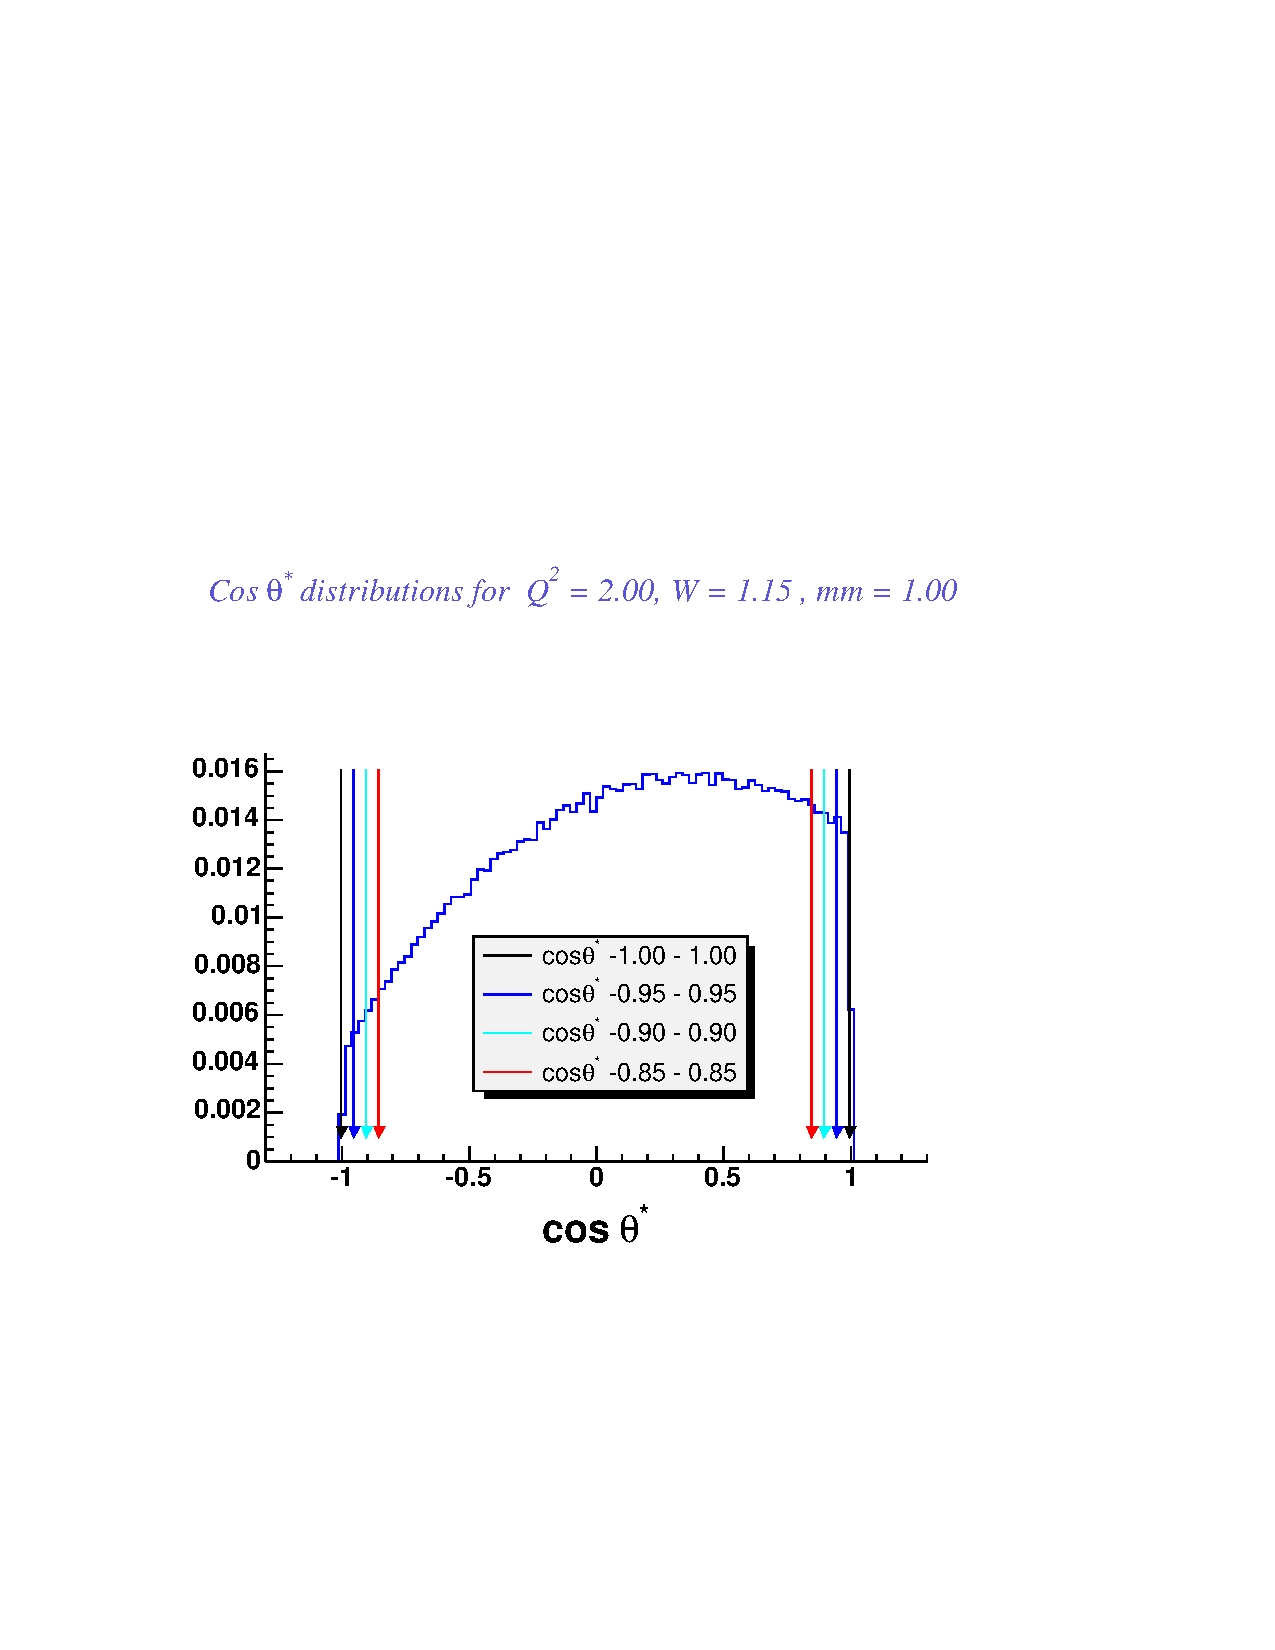
\includegraphics[width = 11cm, bb = 80 150 500 520]{systematics/img/ccuts}
  \caption{ Different cuts for $\cos\theta^*$ as shown in Table \ref{tab:costheta_cuts}. 
            The distribution comes from the MonteCarlo reconstructed events, and it's normalized to $1$.}
  \label{fig:ccuts}
 \end{center}
\end{figure} 


The variation of the ratios $R_{EM}$ and $R_{SM}$ for the first and second cut is illustrated in 
\F{fig:ratios_cc_syst}.
\begin{figure}[h]
 \begin{center}
  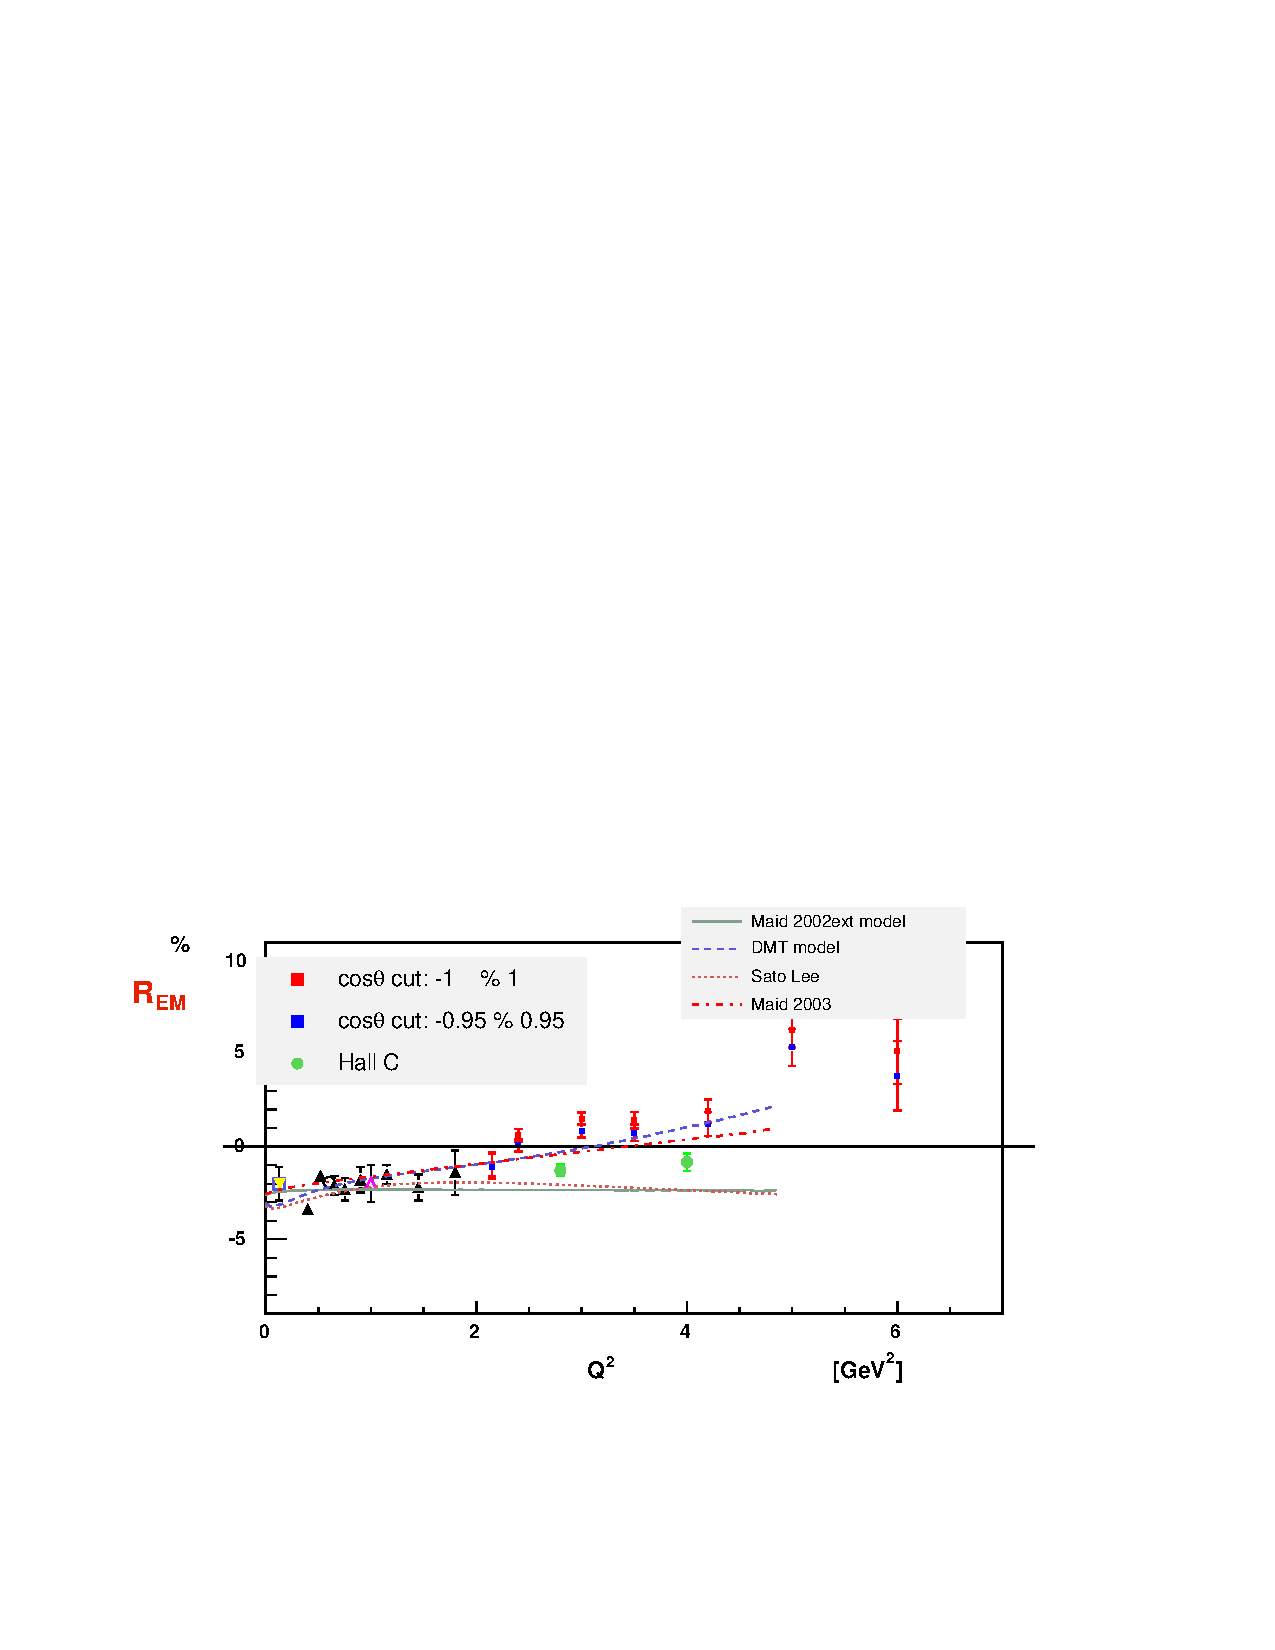
\includegraphics[width = 12cm, bb = 50 120 540 440]{systematics/img/rem_ccsyst}
  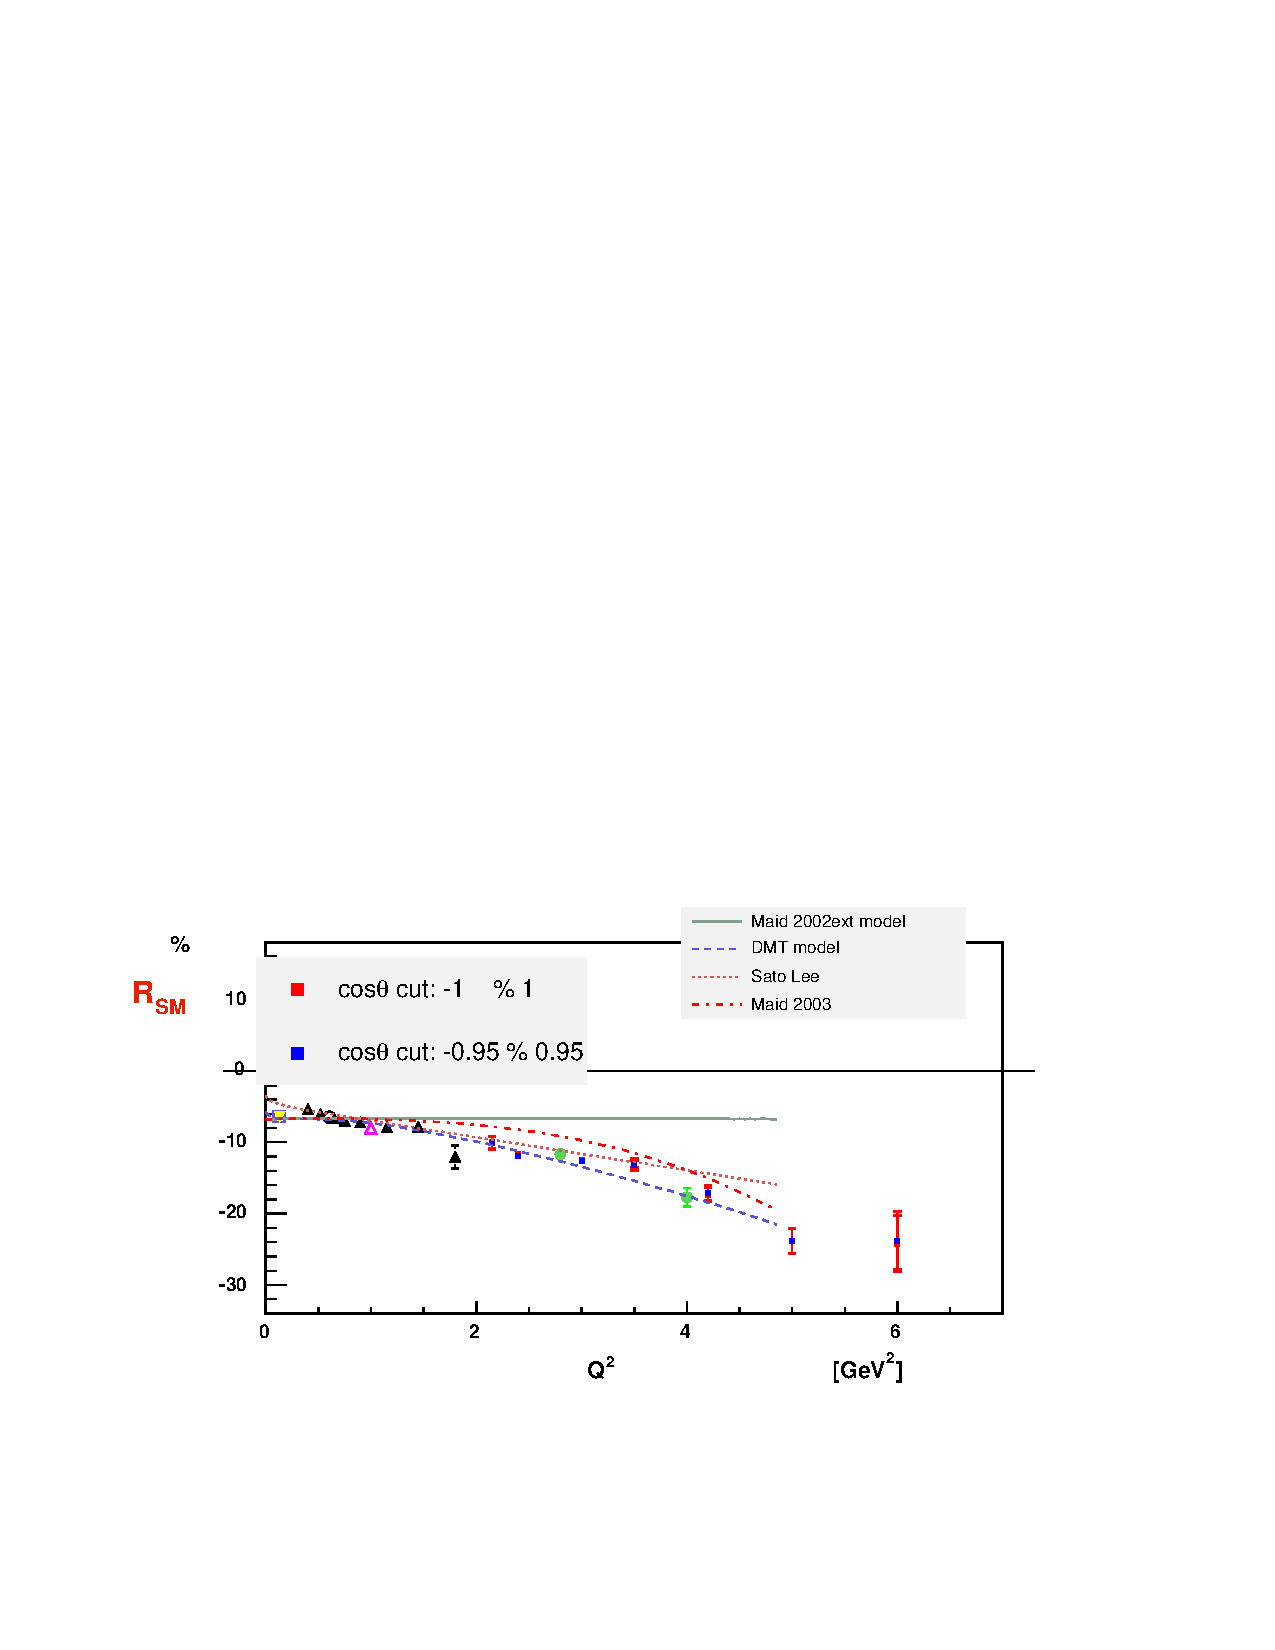
\includegraphics[width = 12cm, bb = 50 100 540 440]{systematics/img/rsm_ccsyst}
  \caption{ Variation of the ratios $R_{EM}$ (top) and $R_{SM}$ (bottom) for the $\cos\theta^*$ cuts:
           $-1 < \cos\theta^* < 1$ and  $-0.95 < \cos\theta^* < 0.95$. }
  \label{fig:ratios_cc_syst}
 \end{center}
\end{figure} 




















\cia\vspace{-2cm}
\section{$\chi^2$ plots for the systematic studies}
See    \begin{verbatim} 
http://www.jlab.org/~ungaro/pi0eprod/bin_ave
\end{verbatim}
for the $\chi^2$ distributions for different cuts in missing mass and $\cos\theta^*$
and for Lorentz/Invariant method.


%\section{Fiducial Cuts}
%\input{analysis/l.tex}




